\documentclass{article}

\usepackage{csvsimple}
\usepackage{graphicx}
\usepackage{longtable}
\usepackage{booktabs}

\makeatletter
\newcommand*{\centerfloat}{%
  \parindent \z@
  \leftskip \z@ \@plus 1fil \@minus \textwidth
  \rightskip\leftskip
  \parfillskip \z@skip}
\makeatother

\begin{document}

\begin{table}
    \centering
    \caption{Classification accuracy in the last decade in time period.}
    \csvautobooktabular{end_year_results.csv}
\end{table}

\begin{table}
    \centering
    \caption{Average classification accuracy over all decades.}
    \csvautobooktabular{year_average_results.csv}
\end{table}

\csvautobooklongtable{all_models.csv}

\begin{figure}
    \centerfloat
    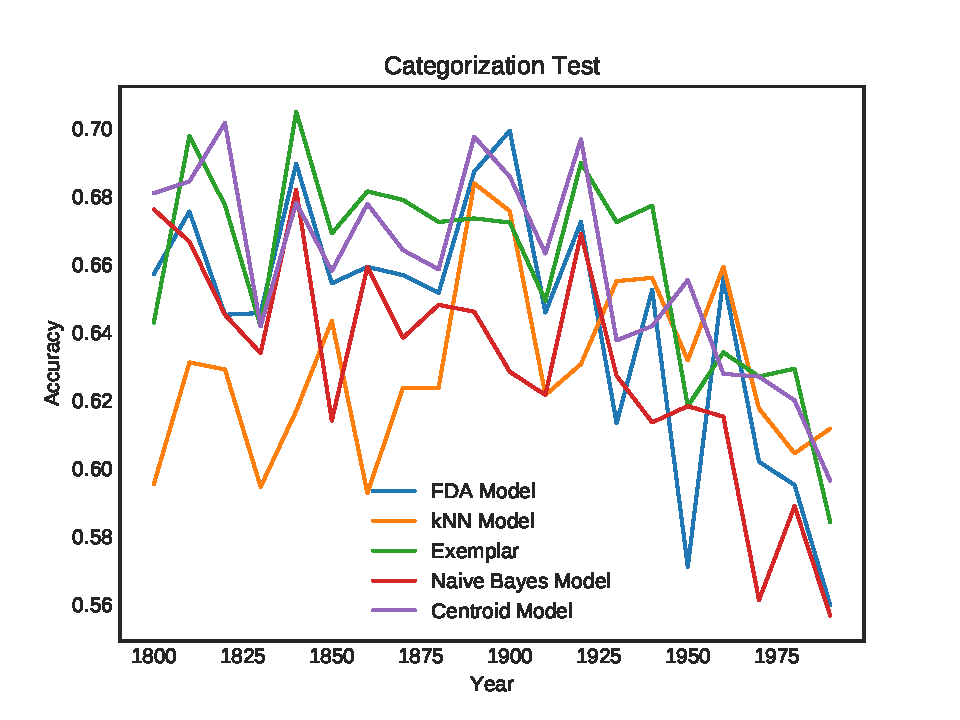
\includegraphics[width=1.75\linewidth]{results_categorization_test.pdf}
    \caption{Categorization test.}
\end{figure}

\begin{figure}
    \centerfloat
    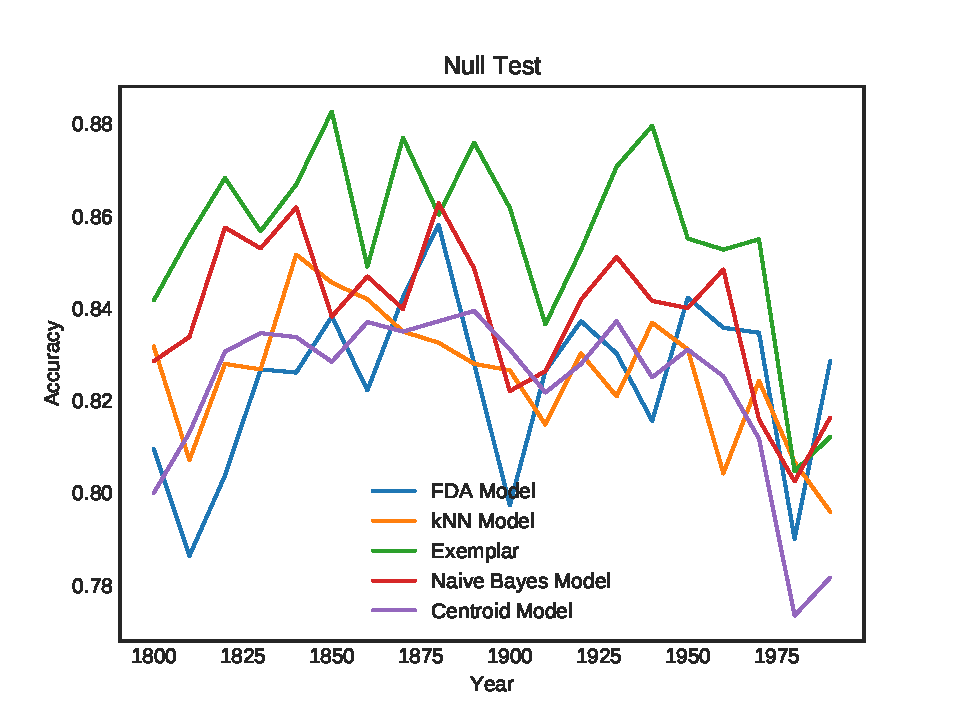
\includegraphics[width=1.75\linewidth]{results_null_test.pdf}
    \caption{Null test.}
\end{figure}

\begin{figure}
    \centerfloat
    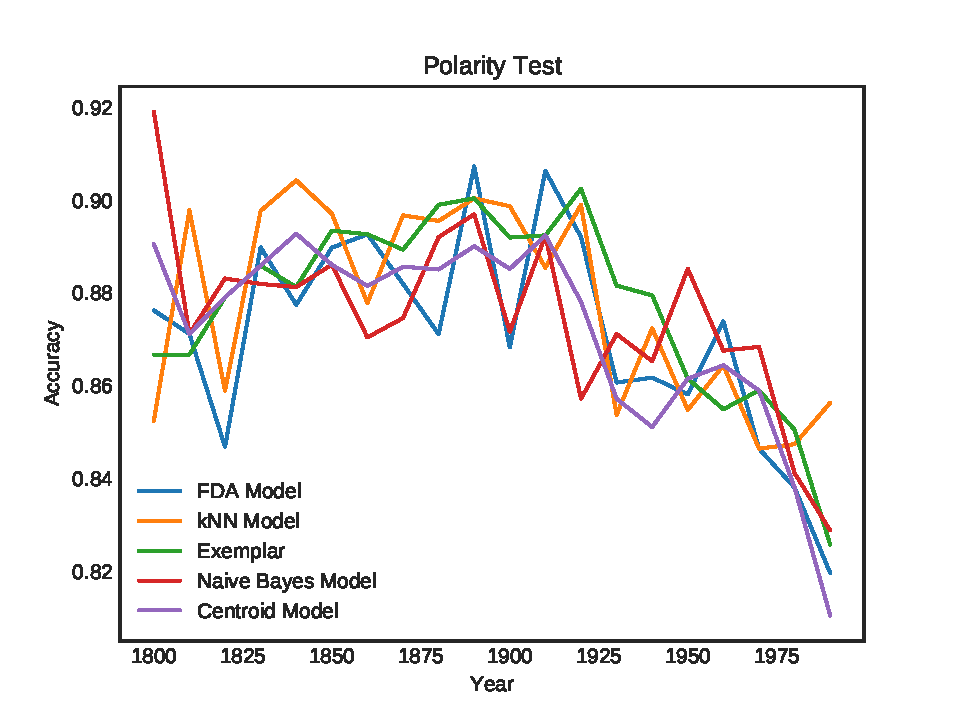
\includegraphics[width=1.75\linewidth]{results_polarity_test.pdf}
    \caption{Polarity test.}
\end{figure}

\end{document}
